\documentclass[]{article}
\usepackage{lmodern}
\usepackage{amssymb,amsmath}
\usepackage{ifxetex,ifluatex}
\usepackage{fixltx2e} % provides \textsubscript
\ifnum 0\ifxetex 1\fi\ifluatex 1\fi=0 % if pdftex
  \usepackage[T1]{fontenc}
  \usepackage[utf8]{inputenc}
\else % if luatex or xelatex
  \ifxetex
    \usepackage{mathspec}
  \else
    \usepackage{fontspec}
  \fi
  \defaultfontfeatures{Ligatures=TeX,Scale=MatchLowercase}
\fi
% use upquote if available, for straight quotes in verbatim environments
\IfFileExists{upquote.sty}{\usepackage{upquote}}{}
% use microtype if available
\IfFileExists{microtype.sty}{%
\usepackage{microtype}
\UseMicrotypeSet[protrusion]{basicmath} % disable protrusion for tt fonts
}{}
\usepackage[margin=1in]{geometry}
\usepackage{hyperref}
\hypersetup{unicode=true,
            pdftitle={FlipTheFleet Black Box Data Tests},
            pdfauthor={Ben Anderson (b.anderson@soton.ac.uk, @dataknut)},
            pdfborder={0 0 0},
            breaklinks=true}
\urlstyle{same}  % don't use monospace font for urls
\usepackage{color}
\usepackage{fancyvrb}
\newcommand{\VerbBar}{|}
\newcommand{\VERB}{\Verb[commandchars=\\\{\}]}
\DefineVerbatimEnvironment{Highlighting}{Verbatim}{commandchars=\\\{\}}
% Add ',fontsize=\small' for more characters per line
\usepackage{framed}
\definecolor{shadecolor}{RGB}{248,248,248}
\newenvironment{Shaded}{\begin{snugshade}}{\end{snugshade}}
\newcommand{\KeywordTok}[1]{\textcolor[rgb]{0.13,0.29,0.53}{\textbf{#1}}}
\newcommand{\DataTypeTok}[1]{\textcolor[rgb]{0.13,0.29,0.53}{#1}}
\newcommand{\DecValTok}[1]{\textcolor[rgb]{0.00,0.00,0.81}{#1}}
\newcommand{\BaseNTok}[1]{\textcolor[rgb]{0.00,0.00,0.81}{#1}}
\newcommand{\FloatTok}[1]{\textcolor[rgb]{0.00,0.00,0.81}{#1}}
\newcommand{\ConstantTok}[1]{\textcolor[rgb]{0.00,0.00,0.00}{#1}}
\newcommand{\CharTok}[1]{\textcolor[rgb]{0.31,0.60,0.02}{#1}}
\newcommand{\SpecialCharTok}[1]{\textcolor[rgb]{0.00,0.00,0.00}{#1}}
\newcommand{\StringTok}[1]{\textcolor[rgb]{0.31,0.60,0.02}{#1}}
\newcommand{\VerbatimStringTok}[1]{\textcolor[rgb]{0.31,0.60,0.02}{#1}}
\newcommand{\SpecialStringTok}[1]{\textcolor[rgb]{0.31,0.60,0.02}{#1}}
\newcommand{\ImportTok}[1]{#1}
\newcommand{\CommentTok}[1]{\textcolor[rgb]{0.56,0.35,0.01}{\textit{#1}}}
\newcommand{\DocumentationTok}[1]{\textcolor[rgb]{0.56,0.35,0.01}{\textbf{\textit{#1}}}}
\newcommand{\AnnotationTok}[1]{\textcolor[rgb]{0.56,0.35,0.01}{\textbf{\textit{#1}}}}
\newcommand{\CommentVarTok}[1]{\textcolor[rgb]{0.56,0.35,0.01}{\textbf{\textit{#1}}}}
\newcommand{\OtherTok}[1]{\textcolor[rgb]{0.56,0.35,0.01}{#1}}
\newcommand{\FunctionTok}[1]{\textcolor[rgb]{0.00,0.00,0.00}{#1}}
\newcommand{\VariableTok}[1]{\textcolor[rgb]{0.00,0.00,0.00}{#1}}
\newcommand{\ControlFlowTok}[1]{\textcolor[rgb]{0.13,0.29,0.53}{\textbf{#1}}}
\newcommand{\OperatorTok}[1]{\textcolor[rgb]{0.81,0.36,0.00}{\textbf{#1}}}
\newcommand{\BuiltInTok}[1]{#1}
\newcommand{\ExtensionTok}[1]{#1}
\newcommand{\PreprocessorTok}[1]{\textcolor[rgb]{0.56,0.35,0.01}{\textit{#1}}}
\newcommand{\AttributeTok}[1]{\textcolor[rgb]{0.77,0.63,0.00}{#1}}
\newcommand{\RegionMarkerTok}[1]{#1}
\newcommand{\InformationTok}[1]{\textcolor[rgb]{0.56,0.35,0.01}{\textbf{\textit{#1}}}}
\newcommand{\WarningTok}[1]{\textcolor[rgb]{0.56,0.35,0.01}{\textbf{\textit{#1}}}}
\newcommand{\AlertTok}[1]{\textcolor[rgb]{0.94,0.16,0.16}{#1}}
\newcommand{\ErrorTok}[1]{\textcolor[rgb]{0.64,0.00,0.00}{\textbf{#1}}}
\newcommand{\NormalTok}[1]{#1}
\usepackage{longtable,booktabs}
\usepackage{graphicx,grffile}
\makeatletter
\def\maxwidth{\ifdim\Gin@nat@width>\linewidth\linewidth\else\Gin@nat@width\fi}
\def\maxheight{\ifdim\Gin@nat@height>\textheight\textheight\else\Gin@nat@height\fi}
\makeatother
% Scale images if necessary, so that they will not overflow the page
% margins by default, and it is still possible to overwrite the defaults
% using explicit options in \includegraphics[width, height, ...]{}
\setkeys{Gin}{width=\maxwidth,height=\maxheight,keepaspectratio}
\IfFileExists{parskip.sty}{%
\usepackage{parskip}
}{% else
\setlength{\parindent}{0pt}
\setlength{\parskip}{6pt plus 2pt minus 1pt}
}
\setlength{\emergencystretch}{3em}  % prevent overfull lines
\providecommand{\tightlist}{%
  \setlength{\itemsep}{0pt}\setlength{\parskip}{0pt}}
\setcounter{secnumdepth}{5}
% Redefines (sub)paragraphs to behave more like sections
\ifx\paragraph\undefined\else
\let\oldparagraph\paragraph
\renewcommand{\paragraph}[1]{\oldparagraph{#1}\mbox{}}
\fi
\ifx\subparagraph\undefined\else
\let\oldsubparagraph\subparagraph
\renewcommand{\subparagraph}[1]{\oldsubparagraph{#1}\mbox{}}
\fi

%%% Use protect on footnotes to avoid problems with footnotes in titles
\let\rmarkdownfootnote\footnote%
\def\footnote{\protect\rmarkdownfootnote}

%%% Change title format to be more compact
\usepackage{titling}

% Create subtitle command for use in maketitle
\newcommand{\subtitle}[1]{
  \posttitle{
    \begin{center}\large#1\end{center}
    }
}

\setlength{\droptitle}{-2em}

  \title{FlipTheFleet Black Box Data Tests}
    \pretitle{\vspace{\droptitle}\centering\huge}
  \posttitle{\par}
  \subtitle{Testing Time of Charging}
  \author{Ben Anderson
(\href{mailto:b.anderson@soton.ac.uk}{\nolinkurl{b.anderson@soton.ac.uk}},
\texttt{@dataknut})}
    \preauthor{\centering\large\emph}
  \postauthor{\par}
      \predate{\centering\large\emph}
  \postdate{\par}
    \date{Last run at: 2018-09-17 12:16:32}


\begin{document}
\maketitle

{
\setcounter{tocdepth}{2}
\tableofcontents
}
\newpage

\section{Citation}\label{citation}

If you wish to use any of the material from this report please cite as:

\begin{itemize}
\tightlist
\item
  Anderson, B. (2018) \emph{FlipTheFleet Black Box Data Tests: Testing
  Time of Charging},
  \href{http://www.otago.ac.nz/centre-sustainability/}{Centre for
  Sustainability}, University of Otago: Dunedin.
\end{itemize}

This work is (c) 2018 the University of Southampton. Re-use is governed
by \href{https://github.com/CfSOtago/GREENGrid/blob/master/LICENSE}{this
license}.

\newpage

\section{About}\label{about}

\subsection{Circulation}\label{circulation}

Report circulation:

\begin{itemize}
\tightlist
\item
  Restricted to:
  \href{https://www.otago.ac.nz/centre-sustainability/research/energy/otago050285.html}{NZ
  GREEN Grid} project partners and contractors.
\end{itemize}

\subsection{Purpose}\label{purpose}

This report is intended to:

\begin{itemize}
\tightlist
\item
  load and test preliminary
  `\href{https://flipthefleet.org/ev-black-box/}{black box}' (see Figure
  \ref{fig:blackBox}) EV monitoring data provided for assessment
  purposes by \href{http://flipthefleet.org/}{FlipTheFleet}
\item
  preliminary analysis of time of charging to understand impact on
  `peak' electricity demand
\end{itemize}

\begin{figure}

\hfill{}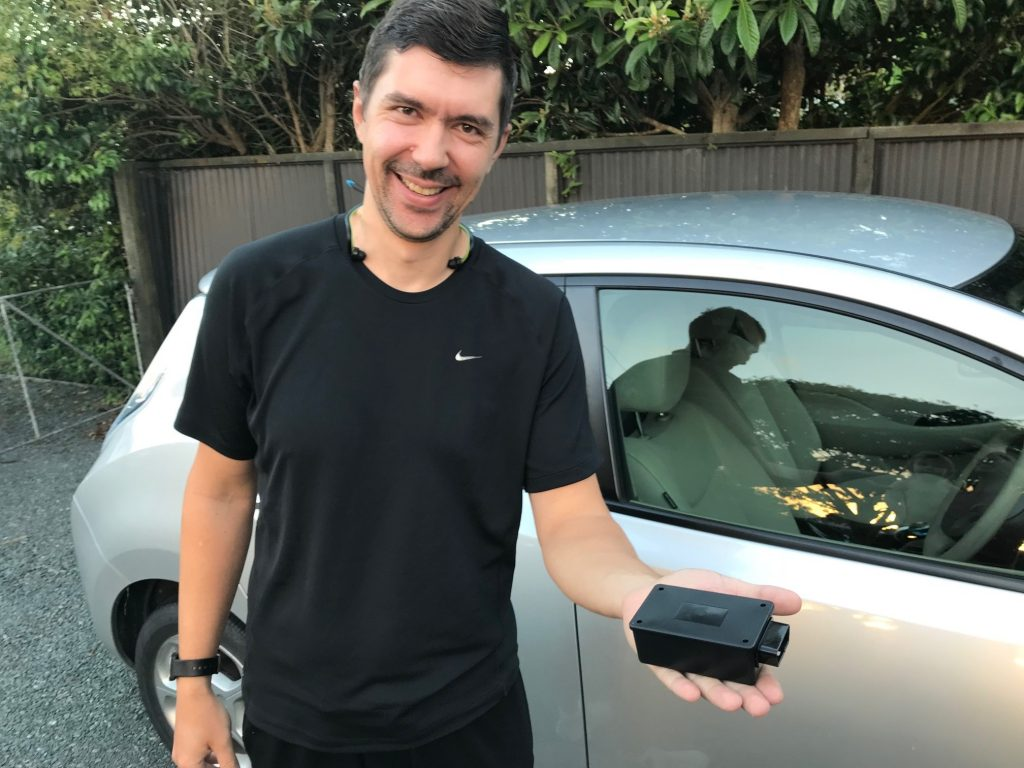
\includegraphics[width=4.24in]{fig/bb} 

\caption{The Black Box (Source: FlipTheFleet)}\label{fig:blackBox}
\end{figure}

\subsection{Requirements:}\label{requirements}

\begin{itemize}
\tightlist
\item
  test FlipTheFleet black box dataset stored on the University of
  Otago's High-Capacity Central File Storage
  \href{https://www.otago.ac.nz/its/services/hosting/otago068353.html}{HCS}
  at: /Volumes/hum-csafe/Research Projects/GREEN
  Grid/externalData/flipTheFleet/
\end{itemize}

\subsection{Code and report history}\label{code-and-report-history}

Generally tracked via our git.soton
\href{https://git.soton.ac.uk/ba1e12/nzGREENGrid}{repo}:

\begin{itemize}
\tightlist
\item
  \href{https://git.soton.ac.uk/ba1e12/nzGREENGrid/commits/master}{history}
\item
  \href{https://git.soton.ac.uk/ba1e12/nzGREENGrid/issues}{issues}
\end{itemize}

Specific history of this code:

\begin{itemize}
\tightlist
\item
  \url{https://git.soton.ac.uk/ba1e12/nzGREENGrid/tree/master/analysis/ev}
\end{itemize}

\subsection{Support}\label{support}

This work was supported by:

\begin{itemize}
\tightlist
\item
  The \href{https://www.otago.ac.nz/}{University of Otago};
\item
  The \href{https://www.southampton.ac.uk/}{University of Southampton};
\item
  The New Zealand \href{http://www.mbie.govt.nz/}{Ministry of Business,
  Innovation and Employment (MBIE)} through the
  \href{https://www.otago.ac.nz/centre-sustainability/research/energy/otago050285.html}{NZ
  GREEN Grid} project;
\item
  \href{http://www.energy.soton.ac.uk/tag/spatialec/}{SPATIALEC} - a
  \href{http://ec.europa.eu/research/mariecurieactions/about-msca/actions/if/index_en.htm}{Marie
  Skłodowska-Curie Global Fellowship} based at the University of Otago's
  \href{http://www.otago.ac.nz/centre-sustainability/staff/otago673896.html}{Centre
  for Sustainability} (2017-2019) \& the University of Southampton's
  Sustainable Energy Research Group (2019-202).
\end{itemize}

We do not `support' the code but if you have a problem check the
\href{https://git.soton.ac.uk/ba1e12/nzGREENGrid/issues}{issues} on our
\href{https://git.soton.ac.uk/ba1e12/nzGREENGrid}{repo} and if it
doesn't already exist, open one. We might be able to fix it :-)

\subsection{Notes}\label{notes}

This document was created using
\href{https://cran.r-project.org/package=knitr}{knitr} in
\href{http://www.rstudio.com}{RStudio} with R version 3.5.1 (2018-07-02)
running on x86\_64-apple-darwin15.6.0. Some of the R code has been
included where used for information and reference purposes. Full code is
\href{https://github.com/CfSOtago/GREENGrid/tree/master/analysis/ev}{available}
as noted above.

\section{Load and check data}\label{load-and-check-data}

\subsection{Load data}\label{load-data}

In this section we load and describe the data from
/Volumes/hum-csafe/Research Projects/GREEN
Grid/externalData/flipTheFleet/EVBlackBox export 2018-06-10-233146.csv.
First we load the data.

\begin{Shaded}
\begin{Highlighting}[]
\NormalTok{ftfDT <-}\StringTok{ }\NormalTok{data.table}\OperatorTok{::}\KeywordTok{as.data.table}\NormalTok{(readr}\OperatorTok{::}\KeywordTok{read_csv}\NormalTok{(ggParams}\OperatorTok{$}\NormalTok{ftfFile))}
\end{Highlighting}
\end{Shaded}

\begin{verbatim}
## Parsed with column specification:
## cols(
##   .default = col_integer(),
##   `Reg No` = col_character(),
##   `Date (GPS)` = col_character(),
##   `Time (GPS)` = col_time(format = ""),
##   Latitude = col_double(),
##   Longitude = col_double(),
##   Altitude = col_double(),
##   `Speed (GPS)` = col_double(),
##   `Speed (Speedometer)` = col_double(),
##   `Course (deg)` = col_double(),
##   SOC = col_double(),
##   AHr = col_double(),
##   `Pack volts` = col_double(),
##   `Pack amps` = col_double(),
##   `Pack 1 temp (C)` = col_double(),
##   `Pack 2 temp (C)` = col_double(),
##   `Pack 3 temp (C)` = col_double(),
##   `Pack 4 temp (C)` = col_double(),
##   `12V battery (amps)` = col_double(),
##   Hx = col_double(),
##   VIN = col_character()
##   # ... with 16 more columns
## )
\end{verbatim}

\begin{verbatim}
## See spec(...) for full column specifications.
\end{verbatim}

That loaded 12,487 observations.

\subsection{Create derived variables}\label{create-derived-variables}

Next we create some useful derived variables. Errors may be `odd' dates
and times or even not set in the original data as we see below.

\begin{Shaded}
\begin{Highlighting}[]
\CommentTok{# create derived variables}
\NormalTok{ftfDT <-}\StringTok{ }\KeywordTok{createDerivedFtF}\NormalTok{(ftfDT)}
\end{Highlighting}
\end{Shaded}

\begin{verbatim}
## Warning: 1160 failed to parse.
\end{verbatim}

\begin{Shaded}
\begin{Highlighting}[]
\NormalTok{t <-}\StringTok{ }\NormalTok{ftfDT[}\KeywordTok{is.na}\NormalTok{(rDate), .(}\DataTypeTok{nObs =}\NormalTok{ .N,}
                           \DataTypeTok{meanPackVolts =} \KeywordTok{mean}\NormalTok{(}\StringTok{`}\DataTypeTok{Pack volts}\StringTok{`}\NormalTok{)), }
\NormalTok{           keyby =}\StringTok{ }\NormalTok{.(}\StringTok{`}\DataTypeTok{Date (GPS)}\StringTok{`}\NormalTok{, }\StringTok{`}\DataTypeTok{Time (GPS)}\StringTok{`}\NormalTok{)]}

\NormalTok{knitr}\OperatorTok{::}\KeywordTok{kable}\NormalTok{(}\DataTypeTok{caption =} \StringTok{"Number of obs and mean pack volts where date cannot be set by original GPS Date & Time"}\NormalTok{, t)}
\end{Highlighting}
\end{Shaded}

\begin{table}[t]

\caption{(\#tab:process ftf data)Number of obs and mean pack volts where date cannot be set by original GPS Date & Time}
\centering
\begin{tabular}{l|l|r|r}
\hline
Date (GPS) & Time (GPS) & nObs & meanPackVolts\\
\hline
NA & NA & 1160 & 372.2431\\
\hline
\end{tabular}
\end{table}

\begin{Shaded}
\begin{Highlighting}[]
\NormalTok{t <-}\StringTok{ }\NormalTok{ftfDT[}\KeywordTok{is.na}\NormalTok{(rTime), .(}\DataTypeTok{nObs =}\NormalTok{ .N,}
                           \DataTypeTok{meanPackVolts =} \KeywordTok{mean}\NormalTok{(}\StringTok{`}\DataTypeTok{Pack volts}\StringTok{`}\NormalTok{)), }
\NormalTok{           keyby =}\StringTok{ }\NormalTok{.(}\StringTok{`}\DataTypeTok{Date (GPS)}\StringTok{`}\NormalTok{, }\StringTok{`}\DataTypeTok{Time (GPS)}\StringTok{`}\NormalTok{)]}

\NormalTok{knitr}\OperatorTok{::}\KeywordTok{kable}\NormalTok{(}\DataTypeTok{caption =} \StringTok{"Number of obs and mean pack volts where time cannot be set by original GPS Date & Time"}\NormalTok{, t)}
\end{Highlighting}
\end{Shaded}

\begin{table}[t]

\caption{(\#tab:process ftf data)Number of obs and mean pack volts where time cannot be set by original GPS Date & Time}
\centering
\begin{tabular}{l|l|r|r}
\hline
Date (GPS) & Time (GPS) & nObs & meanPackVolts\\
\hline
NA & NA & 1160 & 372.2431\\
\hline
\end{tabular}
\end{table}

We remove these NAs from the data

\begin{quote}
\emph{XX (should we - what does GPS NA mean? no signal?) XX }
\end{quote}

Doing so removed 1160 (9.29 \%) observations.

\subsection{Location inference}\label{location-inference}

Figure \ref{fig:mapAllLocations} maps the location of a subset of the
observations in the dataset coloured by \texttt{Speed\ (GPS)}. If we
selected just one vehicle and zoomed our map to the location at 01:00 -
04:00 when speed is 0 then we would probably determine their home. We
could also determine other places visited at other times\ldots{} This
indicates how
\href{http://toddwschneider.com/posts/analyzing-1-1-billion-nyc-taxi-and-uber-trips-with-a-vengeance/}{disclosive
GPS Lat/Long can be} even if address data is not provided.

\begin{verbatim}
## Warning: bounding box given to google - spatial extent only approximate.
\end{verbatim}

\begin{verbatim}
## converting bounding box to center/zoom specification. (experimental)
\end{verbatim}

\begin{verbatim}
## Map from URL : http://maps.googleapis.com/maps/api/staticmap?center=-36.729092,174.727632&zoom=12&size=640x640&scale=2&maptype=terrain&language=en-EN&sensor=false
\end{verbatim}

\begin{verbatim}
## Scale for 'x' is already present. Adding another scale for 'x', which
## will replace the existing scale.
\end{verbatim}

\begin{verbatim}
## Scale for 'y' is already present. Adding another scale for 'y', which
## will replace the existing scale.
\end{verbatim}

\begin{verbatim}
## Warning: Removed 10172 rows containing missing values (geom_point).
\end{verbatim}

\begin{figure}
\centering
\includegraphics{ftFBlackBoxTestDataChargeTime_files/figure-latex/mapAllLocations-1.pdf}
\caption{\label{fig:mapAllLocations}Map of all observations coloured by
speed}
\end{figure}

To avoid any risk of such disclosure we next infer a very coarse
geo-location at each time point so that we can remove the potentially
disclosive GPS data before moving on to the analysis.

Note that this does not necessarily render this dataset \emph{safe}
(\href{https://www.ukdataservice.ac.uk/manage-data/legal-ethical/anonymisation}{anonymised})
as there may well be other variables that provide sufficient information
either on their own or together which would
\href{https://www.ukdataservice.ac.uk/manage-data/legal-ethical/anonymisation}{enable
identification} of the car and it's owner.

\begin{Shaded}
\begin{Highlighting}[]
\NormalTok{ftfDT <-}\StringTok{ }\KeywordTok{inferLocationFtF}\NormalTok{(ftfDT)}

\NormalTok{plotDT <-}\StringTok{ }\NormalTok{ftfDT[, .(}\DataTypeTok{nObs =}\NormalTok{ .N), }
\NormalTok{                keyby =}\StringTok{ }\NormalTok{.(geoLoc, obsHour, rDow)]}

\KeywordTok{ggplot}\NormalTok{(plotDT, }\KeywordTok{aes}\NormalTok{(}\DataTypeTok{x =}\NormalTok{ obsHour, }\DataTypeTok{y =}\NormalTok{ nObs)) }\OperatorTok{+}\StringTok{ }
\StringTok{  }\KeywordTok{geom_col}\NormalTok{() }\OperatorTok{+}\StringTok{ }
\StringTok{  }\KeywordTok{facet_grid}\NormalTok{(rDow }\OperatorTok{~}\StringTok{ }\NormalTok{geoLoc)}
\end{Highlighting}
\end{Shaded}

\begin{figure}
\centering
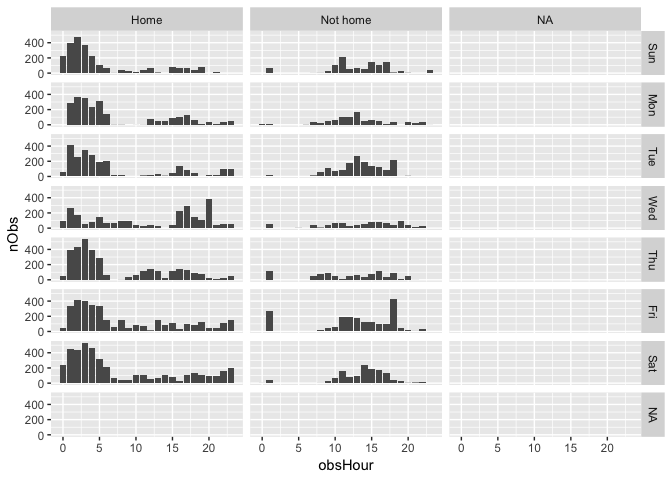
\includegraphics{ftFBlackBoxTestDataChargeTime_files/figure-latex/inferLoc-1.pdf}
\caption{\label{fig:inferLoc}Check inferred location}
\end{figure}

Figure \ref{fig:inferLoc} shows the results of this inference. Does it
look like a reasonable guestimate of location?

\subsection{Make safe dataset}\label{make-safe-dataset}

Next we remove the following variables as they are potentially
disclosive:

\begin{itemize}
\tightlist
\item
  \texttt{Reg\ No} - this is converted to \texttt{evID} using an
  encryption method
\item
  \texttt{Latitude}
\item
  \texttt{Longitude}
\item
  \texttt{Course\ (deg)}
\end{itemize}

The remaining variables are described in detail in
\href{https://www.dropbox.com/s/bfepx3sgfxek78e/ftFBlackBoxTestDataCodebook.docx?dl=0}{ftFBlackBoxTestDataCodebook.docx}.

\subsection{Check variables of interest for this
analysis}\label{check-variables-of-interest-for-this-analysis}

Check charger related variables. We think these are:

\begin{itemize}
\tightlist
\item
  \texttt{Charger\ (amps)}
\item
  \texttt{Charger\ (V)}
\end{itemize}

Multiplying these two will give power in W. Figures \ref{fig:checkAmps}
to \ref{fig:checkPower} examine the distribution of amps, volts and the
derived W.

\begin{figure}
\centering
\includegraphics{ftFBlackBoxTestDataChargeTime_files/figure-latex/checkAmps-1.pdf}
\caption{\label{fig:checkAmps}Distribution of charger amp readings}
\end{figure}

\begin{figure}
\centering
\includegraphics{ftFBlackBoxTestDataChargeTime_files/figure-latex/checkVolts-1.pdf}
\caption{\label{fig:checkVolts}Distribution of charger volt readings}
\end{figure}

\begin{figure}
\centering
\includegraphics{ftFBlackBoxTestDataChargeTime_files/figure-latex/checkPower-1.pdf}
\caption{\label{fig:checkPower}Distribution of derived power demand}
\end{figure}

The following table sumarises these distributions.

\begin{table}[t]

\caption{\label{tab:summaryTable}Summary of Charger (amps)}
\centering
\begin{tabular}{l|l|l|l}
\hline
  & Charger (amps) &  Charger (V) &     powerW\\
\hline
 & Min.   : 0.00 & Min.   :  0.000 & Min.   :   0.00\\
\hline
 & 1st Qu.:15.56 & 1st Qu.:  5.711 & 1st Qu.:  89.23\\
\hline
 & Median :15.62 & Median :239.094 & Median :3733.15\\
\hline
 & Mean   :12.05 & Mean   :155.725 & Mean   :2448.08\\
\hline
 & 3rd Qu.:15.62 & 3rd Qu.:241.336 & 3rd Qu.:3768.19\\
\hline
 & Max.   :33.44 & Max.   :249.445 & Max.   :7977.19\\
\hline
\end{tabular}
\end{table}

\emph{XX Is the Amp reading of 33 an outlier? If so should we ignore the
\textasciitilde{}= 8kW values? XX}

\section{Analysis: Timing of
charging}\label{analysis-timing-of-charging}

We assume \texttt{powerW} is a good indicator of charging. For now we do
not exclude the apparent outlier caused by the few very high Amp values
(\texttt{Charger\ (amps)} \textgreater{} 30) but we flag them as
potential problems.

Figure \ref{fig:plotChargingTime} shows mean kW by time of day over the
entire test datset of 39 days from 2018-05-01 to 2018-06-11.

\begin{figure}
\centering
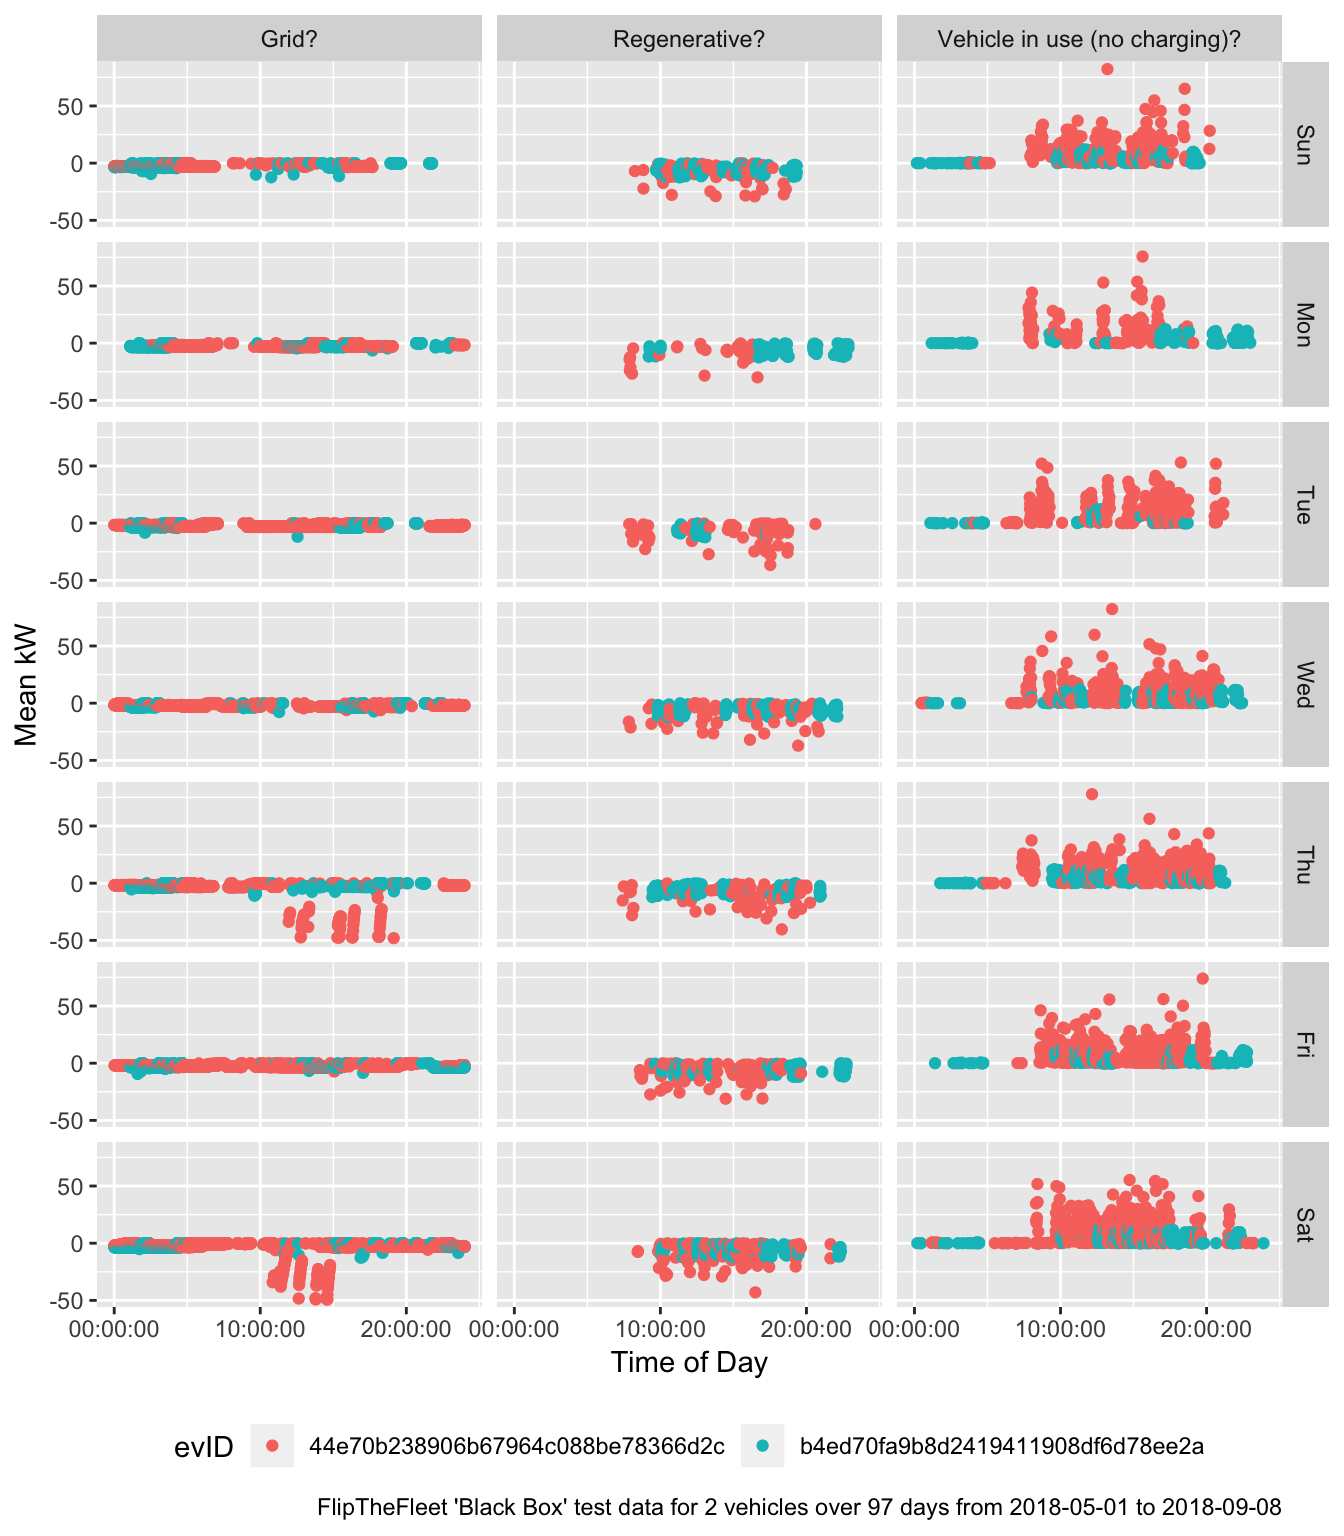
\includegraphics{ftFBlackBoxTestDataChargeTime_files/figure-latex/plotChargingTime-1.pdf}
\caption{\label{fig:plotChargingTime}Inferred charging times and power draw
(all data)}
\end{figure}

Figure \ref{fig:plotChargingTime} seems to show that the very high Amp
values occured on one Sunday and we also appear to see some night
charging `not at home' which may indicate our location inference is
imperfect. We re-draw this plot (Figure \ref{fig:plotChargingTimeClean})
excluding the Amp outliers and also excluding values of exactly 0 for
clarity.

\begin{figure}
\centering
\includegraphics{ftFBlackBoxTestDataChargeTime_files/figure-latex/plotChargingTimeClean-1.pdf}
\caption{\label{fig:plotChargingTimeClean}Inferred charging times and power
draw (outliers and exactly zero values excluded)}
\end{figure}

We can see that this car appears to be on an overnight charging timer at
home although we do still see charging scattered through the rest of the
day.

So where is the non-home charging happening? We need a way to infer
other locations without being disclosive.

\section{Conclusions}\label{conclusions}

Questions to be asked

\begin{itemize}
\tightlist
\item
  Data:

  \begin{itemize}
  \tightlist
  \item
    Do the Amp \& Volt distributions look right?
  \item
    Cause of Amp outliers?
  \item
    Date/Time NA (9.29 \% of observations) are due to a lack of GPS
    date/time (and lat/long). Does this mean that there is no date/time
    in the data when GPS has no signal? Our tests suggest that other
    data (e.g.~power etc) is logged even though there is no date/time.
    Do we need another source of date/time? Could we infer time from
    seconds since powered on (assumes GPS OK at start-up?)?
  \end{itemize}
\item
  Research:

  \begin{itemize}
  \tightlist
  \item
    Do all FlipTheFleet EV owners charge like this?
  \item
    Where are the EVs being charged when not at home and how can we
    tell?
  \item
    Does it vary by car/tariff/commute pattern/main use?
  \item
    What other patterns exist and how much within-vehicle and
    between-vehicle variation is there?
  \end{itemize}
\end{itemize}

\section{Runtime}\label{runtime}

Analysis completed in 25.69 seconds ( 0.43 minutes) using
\href{https://cran.r-project.org/package=knitr}{knitr} in
\href{http://www.rstudio.com}{RStudio} with R version 3.5.1 (2018-07-02)
running on x86\_64-apple-darwin15.6.0.

\section{R environment}\label{r-environment}

R packages used:

\begin{itemize}
\tightlist
\item
  base R - for the basics (R Core Team 2016)
\item
  data.table - for fast (big) data handling (Dowle et al. 2015)
\item
  lubridate - date manipulation (Grolemund and Wickham 2011)
\item
  ggplot2 - for slick graphics (Wickham 2009)
\item
  readr - for csv reading/writing (Wickham, Hester, and Francois 2016)
\item
  openssl - for hashing \texttt{Reg\ No} ({\textbf{???}})
\item
  knitr - to create this document \& neat tables (Xie 2016)
\item
  GREENGrid - for local NZ GREEN Grid project utilities
\end{itemize}

Session info:

\begin{verbatim}
## R version 3.5.1 (2018-07-02)
## Platform: x86_64-apple-darwin15.6.0 (64-bit)
## Running under: macOS High Sierra 10.13.6
## 
## Matrix products: default
## BLAS: /Library/Frameworks/R.framework/Versions/3.5/Resources/lib/libRblas.0.dylib
## LAPACK: /Library/Frameworks/R.framework/Versions/3.5/Resources/lib/libRlapack.dylib
## 
## locale:
## [1] en_GB.UTF-8/en_GB.UTF-8/en_GB.UTF-8/C/en_GB.UTF-8/en_GB.UTF-8
## 
## attached base packages:
## [1] stats     graphics  grDevices utils     datasets  methods   base     
## 
## other attached packages:
## [1] knitr_1.20.13     readr_1.1.1       ggplot2_3.0.0     data.table_1.11.4
## [5] GREENGrid_0.1.0  
## 
## loaded via a namespace (and not attached):
##  [1] tidyselect_0.2.4  xfun_0.3          purrr_0.2.5      
##  [4] reshape2_1.4.3    lattice_0.20-35   colorspace_1.3-2 
##  [7] htmltools_0.3.6   yaml_2.2.0        rlang_0.2.2      
## [10] pillar_1.3.0      glue_1.3.0        withr_2.1.2      
## [13] sp_1.3-1          bindrcpp_0.2.2    jpeg_0.1-8       
## [16] plyr_1.8.4        bindr_0.1.1       stringr_1.3.1    
## [19] munsell_0.5.0     gtable_0.2.0      RgoogleMaps_1.4.2
## [22] mapproj_1.2.6     evaluate_0.11     labeling_0.3     
## [25] highr_0.7         proto_1.0.0       Rcpp_0.12.18     
## [28] geosphere_1.5-7   openssl_1.0.2     scales_1.0.0     
## [31] backports_1.1.2   rjson_0.2.20      hms_0.4.2        
## [34] png_0.1-7         digest_0.6.15     stringi_1.2.4    
## [37] bookdown_0.7      dplyr_0.7.6       grid_3.5.1       
## [40] rprojroot_1.3-2   tools_3.5.1       magrittr_1.5     
## [43] maps_3.3.0        lazyeval_0.2.1    tibble_1.4.2     
## [46] crayon_1.3.4      pkgconfig_2.0.2   lubridate_1.7.4  
## [49] assertthat_0.2.0  rmarkdown_1.10    R6_2.2.2         
## [52] ggmap_2.6.1       compiler_3.5.1
\end{verbatim}

\section*{References}\label{references}
\addcontentsline{toc}{section}{References}

\hypertarget{refs}{}
\hypertarget{ref-data.table}{}
Dowle, M, A Srinivasan, T Short, S Lianoglou with contributions from R
Saporta, and E Antonyan. 2015. \emph{Data.table: Extension of
Data.frame}. \url{https://CRAN.R-project.org/package=data.table}.

\hypertarget{ref-lubridate}{}
Grolemund, Garrett, and Hadley Wickham. 2011. ``Dates and Times Made
Easy with lubridate.'' \emph{Journal of Statistical Software} 40 (3):
1--25. \url{http://www.jstatsoft.org/v40/i03/}.

\hypertarget{ref-baseR}{}
R Core Team. 2016. \emph{R: A Language and Environment for Statistical
Computing}. Vienna, Austria: R Foundation for Statistical Computing.
\url{https://www.R-project.org/}.

\hypertarget{ref-ggplot2}{}
Wickham, Hadley. 2009. \emph{Ggplot2: Elegant Graphics for Data
Analysis}. Springer-Verlag New York. \url{http://ggplot2.org}.

\hypertarget{ref-readr}{}
Wickham, Hadley, Jim Hester, and Romain Francois. 2016. \emph{Readr:
Read Tabular Data}. \url{https://CRAN.R-project.org/package=readr}.

\hypertarget{ref-knitr}{}
Xie, Yihui. 2016. \emph{Knitr: A General-Purpose Package for Dynamic
Report Generation in R}. \url{https://CRAN.R-project.org/package=knitr}.


\end{document}
